\documentclass[twoside]{book}

% Packages required by doxygen
\usepackage{fixltx2e}
\usepackage{calc}
\usepackage{doxygen}
\usepackage[export]{adjustbox} % also loads graphicx
\usepackage{graphicx}
\usepackage[utf8]{inputenc}
\usepackage{makeidx}
\usepackage{multicol}
\usepackage{multirow}
\PassOptionsToPackage{warn}{textcomp}
\usepackage{textcomp}
\usepackage[nointegrals]{wasysym}
\usepackage[table]{xcolor}

% Font selection
\usepackage[T1]{fontenc}
\usepackage[scaled=.90]{helvet}
\usepackage{courier}
\usepackage{amssymb}
\usepackage{sectsty}
\renewcommand{\familydefault}{\sfdefault}
\allsectionsfont{%
  \fontseries{bc}\selectfont%
  \color{darkgray}%
}
\renewcommand{\DoxyLabelFont}{%
  \fontseries{bc}\selectfont%
  \color{darkgray}%
}
\newcommand{\+}{\discretionary{\mbox{\scriptsize$\hookleftarrow$}}{}{}}

% Page & text layout
\usepackage{geometry}
\geometry{%
  a4paper,%
  top=2.5cm,%
  bottom=2.5cm,%
  left=2.5cm,%
  right=2.5cm%
}
\tolerance=750
\hfuzz=15pt
\hbadness=750
\setlength{\emergencystretch}{15pt}
\setlength{\parindent}{0cm}
\setlength{\parskip}{3ex plus 2ex minus 2ex}
\makeatletter
\renewcommand{\paragraph}{%
  \@startsection{paragraph}{4}{0ex}{-1.0ex}{1.0ex}{%
    \normalfont\normalsize\bfseries\SS@parafont%
  }%
}
\renewcommand{\subparagraph}{%
  \@startsection{subparagraph}{5}{0ex}{-1.0ex}{1.0ex}{%
    \normalfont\normalsize\bfseries\SS@subparafont%
  }%
}
\makeatother

% Headers & footers
\usepackage{fancyhdr}
\pagestyle{fancyplain}
\fancyhead[LE]{\fancyplain{}{\bfseries\thepage}}
\fancyhead[CE]{\fancyplain{}{}}
\fancyhead[RE]{\fancyplain{}{\bfseries\leftmark}}
\fancyhead[LO]{\fancyplain{}{\bfseries\rightmark}}
\fancyhead[CO]{\fancyplain{}{}}
\fancyhead[RO]{\fancyplain{}{\bfseries\thepage}}
\fancyfoot[LE]{\fancyplain{}{}}
\fancyfoot[CE]{\fancyplain{}{}}
\fancyfoot[RE]{\fancyplain{}{\bfseries\scriptsize Generated by Doxygen }}
\fancyfoot[LO]{\fancyplain{}{\bfseries\scriptsize Generated by Doxygen }}
\fancyfoot[CO]{\fancyplain{}{}}
\fancyfoot[RO]{\fancyplain{}{}}
\renewcommand{\footrulewidth}{0.4pt}
\renewcommand{\chaptermark}[1]{%
  \markboth{#1}{}%
}
\renewcommand{\sectionmark}[1]{%
  \markright{\thesection\ #1}%
}

% Indices & bibliography
\usepackage{natbib}
\usepackage[titles]{tocloft}
\setcounter{tocdepth}{3}
\setcounter{secnumdepth}{5}
\makeindex

% Hyperlinks (required, but should be loaded last)
\usepackage{ifpdf}
\ifpdf
  \usepackage[pdftex,pagebackref=true]{hyperref}
\else
  \usepackage[ps2pdf,pagebackref=true]{hyperref}
\fi
\hypersetup{%
  colorlinks=true,%
  linkcolor=blue,%
  citecolor=blue,%
  unicode%
}

% Custom commands
\newcommand{\clearemptydoublepage}{%
  \newpage{\pagestyle{empty}\cleardoublepage}%
}

\usepackage{caption}
\captionsetup{labelsep=space,justification=centering,font={bf},singlelinecheck=off,skip=4pt,position=top}

%===== C O N T E N T S =====

\begin{document}

% Titlepage & ToC
\hypersetup{pageanchor=false,
             bookmarksnumbered=true,
             pdfencoding=unicode
            }
\pagenumbering{alph}
\begin{titlepage}
\vspace*{7cm}
\begin{center}%
{\Large My Project }\\
\vspace*{1cm}
{\large Generated by Doxygen 1.8.13}\\
\end{center}
\end{titlepage}
\clearemptydoublepage
\pagenumbering{roman}
\tableofcontents
\clearemptydoublepage
\pagenumbering{arabic}
\hypersetup{pageanchor=true}

%--- Begin generated contents ---
\chapter{Class Index}
\section{Class List}
Here are the classes, structs, unions and interfaces with brief descriptions\+:\begin{DoxyCompactList}
\item\contentsline{section}{\hyperlink{classgenerate__2D}{generate\+\_\+2D} }{\pageref{classgenerate__2D}}{}
\item\contentsline{section}{\hyperlink{classgenerate__3D}{generate\+\_\+3D} }{\pageref{classgenerate__3D}}{}
\item\contentsline{section}{\hyperlink{classgenerate__display}{generate\+\_\+display} }{\pageref{classgenerate__display}}{}
\item\contentsline{section}{\hyperlink{classmode__select}{mode\+\_\+select} }{\pageref{classmode__select}}{}
\item\contentsline{section}{\hyperlink{classview2Dto3D}{view2\+Dto3D} }{\pageref{classview2Dto3D}}{}
\item\contentsline{section}{\hyperlink{classview3Dto2D}{view3\+Dto2D} }{\pageref{classview3Dto2D}}{}
\end{DoxyCompactList}

\chapter{File Index}
\section{File List}
Here is a list of all files with brief descriptions\+:\begin{DoxyCompactList}
\item\contentsline{section}{\hyperlink{display_8cpp}{display.\+cpp} }{\pageref{display_8cpp}}{}
\item\contentsline{section}{\hyperlink{mode_8cpp}{mode.\+cpp} }{\pageref{mode_8cpp}}{}
\item\contentsline{section}{\hyperlink{process__2D_8cpp}{process\+\_\+2\+D.\+cpp} }{\pageref{process__2D_8cpp}}{}
\item\contentsline{section}{\hyperlink{process__3D_8cpp}{process\+\_\+3\+D.\+cpp} }{\pageref{process__3D_8cpp}}{}
\item\contentsline{section}{\hyperlink{view2to3_8cpp}{view2to3.\+cpp} }{\pageref{view2to3_8cpp}}{}
\item\contentsline{section}{\hyperlink{view3to2_8cpp}{view3to2.\+cpp} }{\pageref{view3to2_8cpp}}{}
\end{DoxyCompactList}

\chapter{Class Documentation}
\hypertarget{classgenerate__2D}{}\section{generate\+\_\+2D Class Reference}
\label{classgenerate__2D}\index{generate\+\_\+2D@{generate\+\_\+2D}}


Collaboration diagram for generate\+\_\+2D\+:
\nopagebreak
\begin{figure}[H]
\begin{center}
\leavevmode
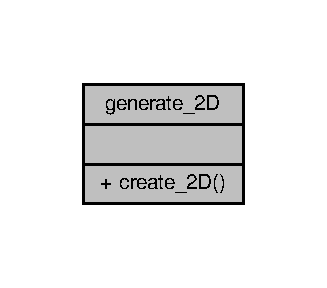
\includegraphics[width=157pt]{classgenerate__2D__coll__graph}
\end{center}
\end{figure}
\subsection*{Public Member Functions}
\begin{DoxyCompactItemize}
\item 
\hyperlink{classgenerate__2D_a8f877568a90f4e5884ff03aa418f1169}{create\+\_\+2D} ()
\end{DoxyCompactItemize}


\subsection{Member Function Documentation}
\mbox{\Hypertarget{classgenerate__2D_a8f877568a90f4e5884ff03aa418f1169}\label{classgenerate__2D_a8f877568a90f4e5884ff03aa418f1169}} 
\index{generate\+\_\+2D@{generate\+\_\+2D}!create\+\_\+2D@{create\+\_\+2D}}
\index{create\+\_\+2D@{create\+\_\+2D}!generate\+\_\+2D@{generate\+\_\+2D}}
\subsubsection{\texorpdfstring{create\+\_\+2\+D()}{create\_2D()}}
{\footnotesize\ttfamily generate\+\_\+2\+D\+::create\+\_\+2D (\begin{DoxyParamCaption}{ }\end{DoxyParamCaption})\hspace{0.3cm}{\ttfamily [inline]}}

This is for providing options to create a 2D graph(having 3 different projections) from files. This function will take a input and store the 2D projections in appropriate data structures. Input can be provided in suitable data structures, such as a array or list of edges and overlapping points in different set of lists or array. The 2D graph generated will be used by different classes.

The documentation for this class was generated from the following file\+:\begin{DoxyCompactItemize}
\item 
\hyperlink{process__2D_8cpp}{process\+\_\+2\+D.\+cpp}\end{DoxyCompactItemize}

\hypertarget{classgenerate__3D}{}\section{generate\+\_\+3D Class Reference}
\label{classgenerate__3D}\index{generate\+\_\+3D@{generate\+\_\+3D}}


Collaboration diagram for generate\+\_\+3D\+:
\nopagebreak
\begin{figure}[H]
\begin{center}
\leavevmode
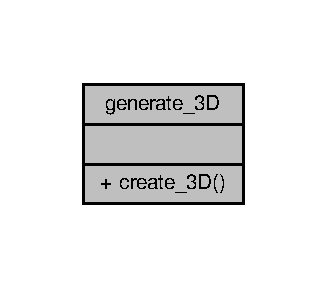
\includegraphics[width=157pt]{classgenerate__3D__coll__graph}
\end{center}
\end{figure}
\subsection*{Public Member Functions}
\begin{DoxyCompactItemize}
\item 
\hyperlink{classgenerate__3D_acd71c91967bb90a72123fd505dcea493}{create\+\_\+3D} ()
\end{DoxyCompactItemize}


\subsection{Member Function Documentation}
\mbox{\Hypertarget{classgenerate__3D_acd71c91967bb90a72123fd505dcea493}\label{classgenerate__3D_acd71c91967bb90a72123fd505dcea493}} 
\index{generate\+\_\+3D@{generate\+\_\+3D}!create\+\_\+3D@{create\+\_\+3D}}
\index{create\+\_\+3D@{create\+\_\+3D}!generate\+\_\+3D@{generate\+\_\+3D}}
\subsubsection{\texorpdfstring{create\+\_\+3\+D()}{create\_3D()}}
{\footnotesize\ttfamily generate\+\_\+3\+D\+::create\+\_\+3D (\begin{DoxyParamCaption}{ }\end{DoxyParamCaption})\hspace{0.3cm}{\ttfamily [inline]}}

This is for putting a 3D graph in proper data structures from a given 3D graph in input file. A 3D graph can be represented as list/array of connected edges and overlapping points. 3D points and edges can be saved in different lists/arrays. These inputs will be saved in proper data stuructures for a 3D graph, and then can be provided to different calsses for further processes.

The documentation for this class was generated from the following file\+:\begin{DoxyCompactItemize}
\item 
\hyperlink{process__3D_8cpp}{process\+\_\+3\+D.\+cpp}\end{DoxyCompactItemize}

\hypertarget{classgenerate__display}{}\section{generate\+\_\+display Class Reference}
\label{classgenerate__display}\index{generate\+\_\+display@{generate\+\_\+display}}


Collaboration diagram for generate\+\_\+display\+:
\nopagebreak
\begin{figure}[H]
\begin{center}
\leavevmode
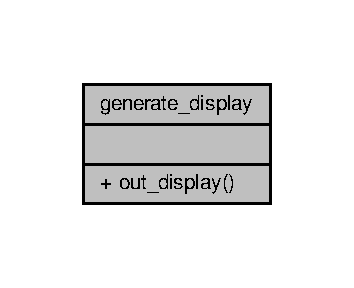
\includegraphics[width=170pt]{classgenerate__display__coll__graph}
\end{center}
\end{figure}
\subsection*{Public Member Functions}
\begin{DoxyCompactItemize}
\item 
\hyperlink{classgenerate__display_a15c857836239ee6642895f284ba44507}{out\+\_\+display} ()
\end{DoxyCompactItemize}


\subsection{Member Function Documentation}
\mbox{\Hypertarget{classgenerate__display_a15c857836239ee6642895f284ba44507}\label{classgenerate__display_a15c857836239ee6642895f284ba44507}} 
\index{generate\+\_\+display@{generate\+\_\+display}!out\+\_\+display@{out\+\_\+display}}
\index{out\+\_\+display@{out\+\_\+display}!generate\+\_\+display@{generate\+\_\+display}}
\subsubsection{\texorpdfstring{out\+\_\+display()}{out\_display()}}
{\footnotesize\ttfamily generate\+\_\+display\+::out\+\_\+display (\begin{DoxyParamCaption}{ }\end{DoxyParamCaption})\hspace{0.3cm}{\ttfamily [inline]}}

This file is for generating the outputs to be showed on screen using U\+Is. The graphs can be converted to different data structures, which can be used to draw visuals or can be given as output files to be stored by useer. The output can be seen as list/array of tuples for 3D graph or different lists for 2D graphs(projections).

The documentation for this class was generated from the following file\+:\begin{DoxyCompactItemize}
\item 
\hyperlink{display_8cpp}{display.\+cpp}\end{DoxyCompactItemize}

\hypertarget{classmode__select}{}\section{mode\+\_\+select Class Reference}
\label{classmode__select}\index{mode\+\_\+select@{mode\+\_\+select}}


Collaboration diagram for mode\+\_\+select\+:
\nopagebreak
\begin{figure}[H]
\begin{center}
\leavevmode
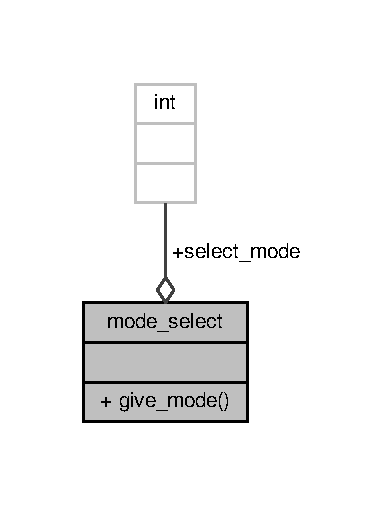
\includegraphics[width=185pt]{classmode__select__coll__graph}
\end{center}
\end{figure}
\subsection*{Public Member Functions}
\begin{DoxyCompactItemize}
\item 
\hyperlink{classmode__select_ad2fbf5488edaa41ff5ab4cbf85e6457a}{give\+\_\+mode} ()
\end{DoxyCompactItemize}
\subsection*{Public Attributes}
\begin{DoxyCompactItemize}
\item 
int \hyperlink{classmode__select_a81b7b37bc5dd126aae4ac9a08270d13a}{select\+\_\+mode}
\end{DoxyCompactItemize}


\subsection{Detailed Description}
User will select mode in this section. 

\subsection{Member Function Documentation}
\mbox{\Hypertarget{classmode__select_ad2fbf5488edaa41ff5ab4cbf85e6457a}\label{classmode__select_ad2fbf5488edaa41ff5ab4cbf85e6457a}} 
\index{mode\+\_\+select@{mode\+\_\+select}!give\+\_\+mode@{give\+\_\+mode}}
\index{give\+\_\+mode@{give\+\_\+mode}!mode\+\_\+select@{mode\+\_\+select}}
\subsubsection{\texorpdfstring{give\+\_\+mode()}{give\_mode()}}
{\footnotesize\ttfamily mode\+\_\+select\+::give\+\_\+mode (\begin{DoxyParamCaption}{ }\end{DoxyParamCaption})\hspace{0.3cm}{\ttfamily [inline]}}

This method is to provide the user to give a input for selecting mode of usages, which can be 3D to 2D or 2D to 3D.\textbackslash{} The input will be taken accordingly and user will be redirected accordingly.

\subsection{Member Data Documentation}
\mbox{\Hypertarget{classmode__select_a81b7b37bc5dd126aae4ac9a08270d13a}\label{classmode__select_a81b7b37bc5dd126aae4ac9a08270d13a}} 
\index{mode\+\_\+select@{mode\+\_\+select}!select\+\_\+mode@{select\+\_\+mode}}
\index{select\+\_\+mode@{select\+\_\+mode}!mode\+\_\+select@{mode\+\_\+select}}
\subsubsection{\texorpdfstring{select\+\_\+mode}{select\_mode}}
{\footnotesize\ttfamily int mode\+\_\+select\+::select\+\_\+mode}



The documentation for this class was generated from the following file\+:\begin{DoxyCompactItemize}
\item 
\hyperlink{mode_8cpp}{mode.\+cpp}\end{DoxyCompactItemize}

\hypertarget{classview2Dto3D}{}\section{view2\+Dto3D Class Reference}
\label{classview2Dto3D}\index{view2\+Dto3D@{view2\+Dto3D}}


Collaboration diagram for view2\+Dto3D\+:
\nopagebreak
\begin{figure}[H]
\begin{center}
\leavevmode
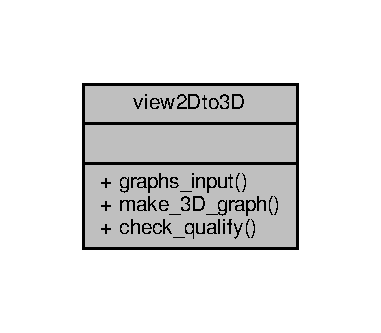
\includegraphics[width=183pt]{classview2Dto3D__coll__graph}
\end{center}
\end{figure}
\subsection*{Public Member Functions}
\begin{DoxyCompactItemize}
\item 
\hyperlink{classview2Dto3D_aeaf8d04a7b6dee4c61a791ddae2d4add}{graphs\+\_\+input} ()
\item 
\hyperlink{classview2Dto3D_a9bb5691d1dae21c9f0fe2573c04db1da}{make\+\_\+3\+D\+\_\+graph} ()
\item 
\hyperlink{classview2Dto3D_a502d119bc3cb39c9c43ce6663e420ce5}{check\+\_\+qualify} ()
\end{DoxyCompactItemize}


\subsection{Member Function Documentation}
\mbox{\Hypertarget{classview2Dto3D_a502d119bc3cb39c9c43ce6663e420ce5}\label{classview2Dto3D_a502d119bc3cb39c9c43ce6663e420ce5}} 
\index{view2\+Dto3D@{view2\+Dto3D}!check\+\_\+qualify@{check\+\_\+qualify}}
\index{check\+\_\+qualify@{check\+\_\+qualify}!view2\+Dto3D@{view2\+Dto3D}}
\subsubsection{\texorpdfstring{check\+\_\+qualify()}{check\_qualify()}}
{\footnotesize\ttfamily view2\+Dto3\+D\+::check\+\_\+qualify (\begin{DoxyParamCaption}{ }\end{DoxyParamCaption})\hspace{0.3cm}{\ttfamily [inline]}}

\mbox{\Hypertarget{classview2Dto3D_aeaf8d04a7b6dee4c61a791ddae2d4add}\label{classview2Dto3D_aeaf8d04a7b6dee4c61a791ddae2d4add}} 
\index{view2\+Dto3D@{view2\+Dto3D}!graphs\+\_\+input@{graphs\+\_\+input}}
\index{graphs\+\_\+input@{graphs\+\_\+input}!view2\+Dto3D@{view2\+Dto3D}}
\subsubsection{\texorpdfstring{graphs\+\_\+input()}{graphs\_input()}}
{\footnotesize\ttfamily view2\+Dto3\+D\+::graphs\+\_\+input (\begin{DoxyParamCaption}{ }\end{DoxyParamCaption})\hspace{0.3cm}{\ttfamily [inline]}}

2D graphs are provided as inputs from file. The following functions of this class can be used to process 2D graphs to generate a 3D graph. This method simply take 2D graphs input to be processed.\mbox{\Hypertarget{classview2Dto3D_a9bb5691d1dae21c9f0fe2573c04db1da}\label{classview2Dto3D_a9bb5691d1dae21c9f0fe2573c04db1da}} 
\index{view2\+Dto3D@{view2\+Dto3D}!make\+\_\+3\+D\+\_\+graph@{make\+\_\+3\+D\+\_\+graph}}
\index{make\+\_\+3\+D\+\_\+graph@{make\+\_\+3\+D\+\_\+graph}!view2\+Dto3D@{view2\+Dto3D}}
\subsubsection{\texorpdfstring{make\+\_\+3\+D\+\_\+graph()}{make\_3D\_graph()}}
{\footnotesize\ttfamily view2\+Dto3\+D\+::make\+\_\+3\+D\+\_\+graph (\begin{DoxyParamCaption}{ }\end{DoxyParamCaption})\hspace{0.3cm}{\ttfamily [inline]}}

Here we convert the provided 2D graphs to a 3D graph. Different projections in 2D graphs will be processed to genrate a 3D graph using the mathematical model planned. Then if a valid 3D graph cannot be obtained form the given projections exception can be showed. Thereafter validity of the 3D graph generated will also be checked, wheather it is the only possible solution or some other solution has been generated. 3D graph generated will be saved in suitable data structure.

The documentation for this class was generated from the following file\+:\begin{DoxyCompactItemize}
\item 
\hyperlink{view2to3_8cpp}{view2to3.\+cpp}\end{DoxyCompactItemize}

\hypertarget{classview3Dto2D}{}\section{view3\+Dto2D Class Reference}
\label{classview3Dto2D}\index{view3\+Dto2D@{view3\+Dto2D}}


Collaboration diagram for view3\+Dto2D\+:
\nopagebreak
\begin{figure}[H]
\begin{center}
\leavevmode
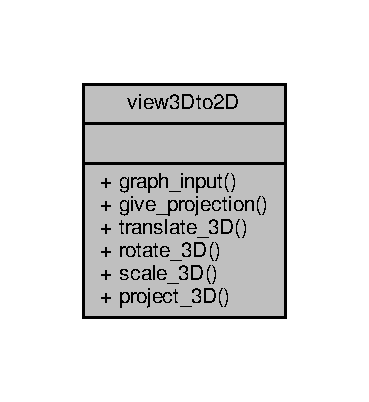
\includegraphics[width=177pt]{classview3Dto2D__coll__graph}
\end{center}
\end{figure}
\subsection*{Public Member Functions}
\begin{DoxyCompactItemize}
\item 
\hyperlink{classview3Dto2D_ab11291f6c3ea5835a15c069ce33c3f9f}{graph\+\_\+input} ()
\item 
\hyperlink{classview3Dto2D_ac598b0f02e0e892f63363ad33bd06ac0}{give\+\_\+projection} ()
\item 
\hyperlink{classview3Dto2D_a9d2c4326ea37b4020ab55e23133105fd}{translate\+\_\+3D} ()
\item 
\hyperlink{classview3Dto2D_a08491d952539c911a02489a500e8f830}{rotate\+\_\+3D} ()
\item 
\hyperlink{classview3Dto2D_a9f4eb503f1f50649fb38df348e1f836b}{scale\+\_\+3D} ()
\item 
\hyperlink{classview3Dto2D_a8b6a91f689534c80d15da1124d69e214}{project\+\_\+3D} ()
\end{DoxyCompactItemize}


\subsection{Member Function Documentation}
\mbox{\Hypertarget{classview3Dto2D_ac598b0f02e0e892f63363ad33bd06ac0}\label{classview3Dto2D_ac598b0f02e0e892f63363ad33bd06ac0}} 
\index{view3\+Dto2D@{view3\+Dto2D}!give\+\_\+projection@{give\+\_\+projection}}
\index{give\+\_\+projection@{give\+\_\+projection}!view3\+Dto2D@{view3\+Dto2D}}
\subsubsection{\texorpdfstring{give\+\_\+projection()}{give\_projection()}}
{\footnotesize\ttfamily view3\+Dto2\+D\+::give\+\_\+projection (\begin{DoxyParamCaption}{ }\end{DoxyParamCaption})\hspace{0.3cm}{\ttfamily [inline]}}

User need to provide planes on which he wants to get 2D projections. Projections can be provided from different transformations on co-\/ordinates axes. For providing a transformated plane user can provide the following.
\begin{DoxyEnumerate}
\item Rotation angles about axes x, y, z.
\item Distance from x, y, z axes.
\item If there is a scaling putted thats too.
\end{DoxyEnumerate}\mbox{\Hypertarget{classview3Dto2D_ab11291f6c3ea5835a15c069ce33c3f9f}\label{classview3Dto2D_ab11291f6c3ea5835a15c069ce33c3f9f}} 
\index{view3\+Dto2D@{view3\+Dto2D}!graph\+\_\+input@{graph\+\_\+input}}
\index{graph\+\_\+input@{graph\+\_\+input}!view3\+Dto2D@{view3\+Dto2D}}
\subsubsection{\texorpdfstring{graph\+\_\+input()}{graph\_input()}}
{\footnotesize\ttfamily view3\+Dto2\+D\+::graph\+\_\+input (\begin{DoxyParamCaption}{ }\end{DoxyParamCaption})\hspace{0.3cm}{\ttfamily [inline]}}

This is the place where all the processing with 3D graph take place. User provide a 3D graph which is required to be converted to 2D, which are projections on any plane.\mbox{\Hypertarget{classview3Dto2D_a8b6a91f689534c80d15da1124d69e214}\label{classview3Dto2D_a8b6a91f689534c80d15da1124d69e214}} 
\index{view3\+Dto2D@{view3\+Dto2D}!project\+\_\+3D@{project\+\_\+3D}}
\index{project\+\_\+3D@{project\+\_\+3D}!view3\+Dto2D@{view3\+Dto2D}}
\subsubsection{\texorpdfstring{project\+\_\+3\+D()}{project\_3D()}}
{\footnotesize\ttfamily view3\+Dto2\+D\+::project\+\_\+3D (\begin{DoxyParamCaption}{ }\end{DoxyParamCaption})\hspace{0.3cm}{\ttfamily [inline]}}

Processed 3D object provided with the projection plane will output the projection of the given object on given plane using this function. user can take output as lists with different 2D projections.\mbox{\Hypertarget{classview3Dto2D_a08491d952539c911a02489a500e8f830}\label{classview3Dto2D_a08491d952539c911a02489a500e8f830}} 
\index{view3\+Dto2D@{view3\+Dto2D}!rotate\+\_\+3D@{rotate\+\_\+3D}}
\index{rotate\+\_\+3D@{rotate\+\_\+3D}!view3\+Dto2D@{view3\+Dto2D}}
\subsubsection{\texorpdfstring{rotate\+\_\+3\+D()}{rotate\_3D()}}
{\footnotesize\ttfamily view3\+Dto2\+D\+::rotate\+\_\+3D (\begin{DoxyParamCaption}{ }\end{DoxyParamCaption})\hspace{0.3cm}{\ttfamily [inline]}}

This function is meant for rotating the 3D object around different axes by angles. It will change the objects data structure in accordance with rules and lemmas stated in mathematical model.\mbox{\Hypertarget{classview3Dto2D_a9f4eb503f1f50649fb38df348e1f836b}\label{classview3Dto2D_a9f4eb503f1f50649fb38df348e1f836b}} 
\index{view3\+Dto2D@{view3\+Dto2D}!scale\+\_\+3D@{scale\+\_\+3D}}
\index{scale\+\_\+3D@{scale\+\_\+3D}!view3\+Dto2D@{view3\+Dto2D}}
\subsubsection{\texorpdfstring{scale\+\_\+3\+D()}{scale\_3D()}}
{\footnotesize\ttfamily view3\+Dto2\+D\+::scale\+\_\+3D (\begin{DoxyParamCaption}{ }\end{DoxyParamCaption})\hspace{0.3cm}{\ttfamily [inline]}}

A 3D object can be scaled for zooming in and out, it will be done using this function.\mbox{\Hypertarget{classview3Dto2D_a9d2c4326ea37b4020ab55e23133105fd}\label{classview3Dto2D_a9d2c4326ea37b4020ab55e23133105fd}} 
\index{view3\+Dto2D@{view3\+Dto2D}!translate\+\_\+3D@{translate\+\_\+3D}}
\index{translate\+\_\+3D@{translate\+\_\+3D}!view3\+Dto2D@{view3\+Dto2D}}
\subsubsection{\texorpdfstring{translate\+\_\+3\+D()}{translate\_3D()}}
{\footnotesize\ttfamily view3\+Dto2\+D\+::translate\+\_\+3D (\begin{DoxyParamCaption}{ }\end{DoxyParamCaption})\hspace{0.3cm}{\ttfamily [inline]}}

For translating a 3D object along coordinate axes. This can be done by changing the object\textquotesingle{}s data structure as per mathematical model.

The documentation for this class was generated from the following file\+:\begin{DoxyCompactItemize}
\item 
\hyperlink{view3to2_8cpp}{view3to2.\+cpp}\end{DoxyCompactItemize}

\chapter{File Documentation}
\hypertarget{display_8cpp}{}\section{display.\+cpp File Reference}
\label{display_8cpp}\index{display.\+cpp@{display.\+cpp}}
{\ttfamily \#include $<$bits/stdc++.\+h$>$}\newline
{\ttfamily \#include $<$Qt\+Gui$>$}\newline
{\ttfamily \#include $<$process\+\_\+3\+D.\+cpp$>$}\newline
{\ttfamily \#include $<$process\+\_\+2\+D.\+cpp$>$}\newline
{\ttfamily \#include $<$view2to3.\+cpp$>$}\newline
{\ttfamily \#include $<$view3to2.\+cpp$>$}\newline
{\ttfamily \#include $<$mode.\+cpp$>$}\newline
Include dependency graph for display.\+cpp\+:
\nopagebreak
\begin{figure}[H]
\begin{center}
\leavevmode
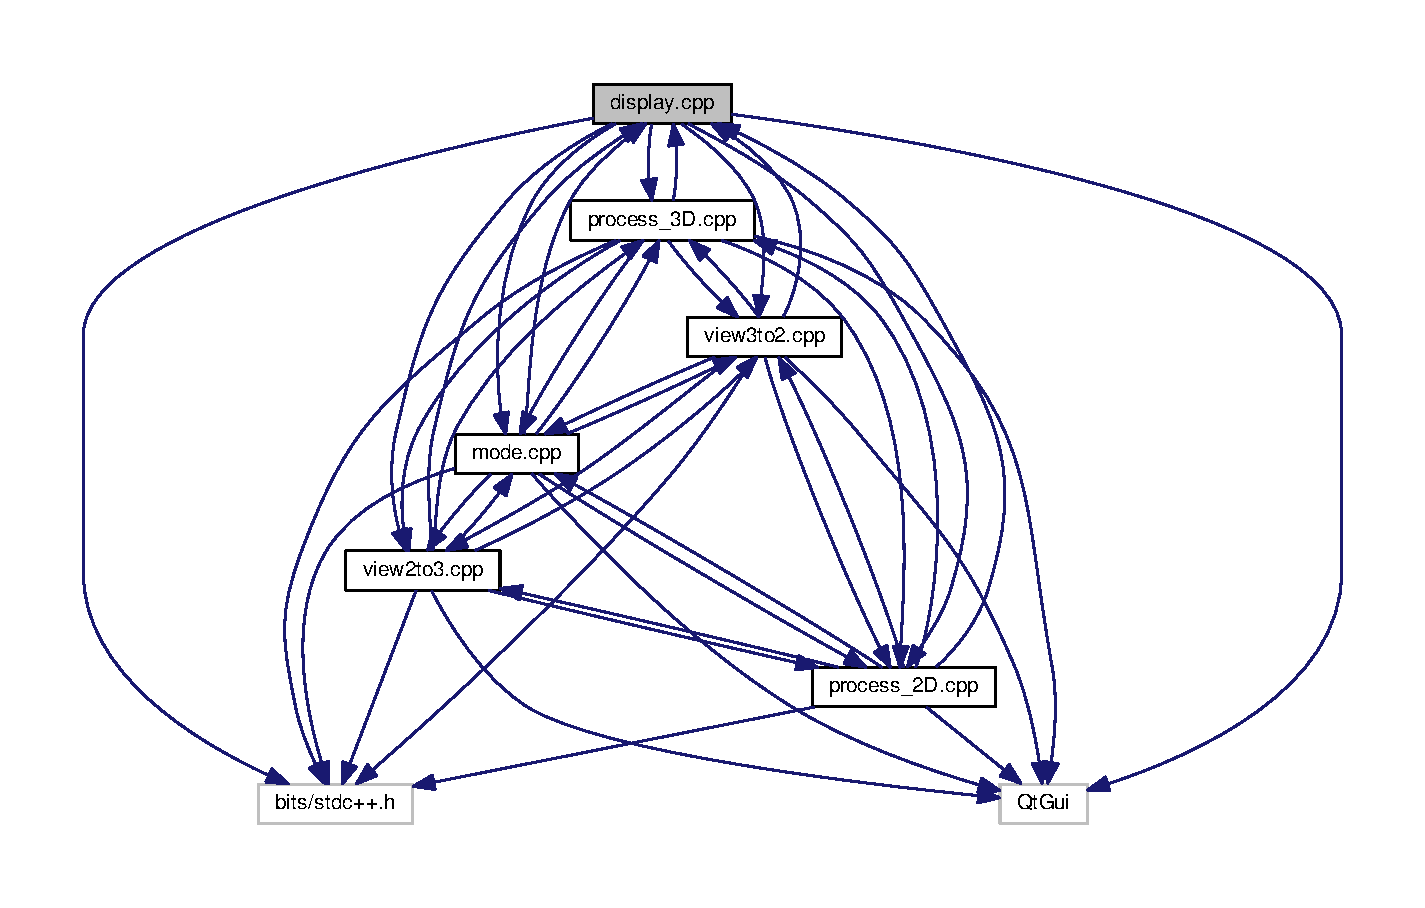
\includegraphics[width=350pt]{display_8cpp__incl}
\end{center}
\end{figure}
This graph shows which files directly or indirectly include this file\+:
\nopagebreak
\begin{figure}[H]
\begin{center}
\leavevmode
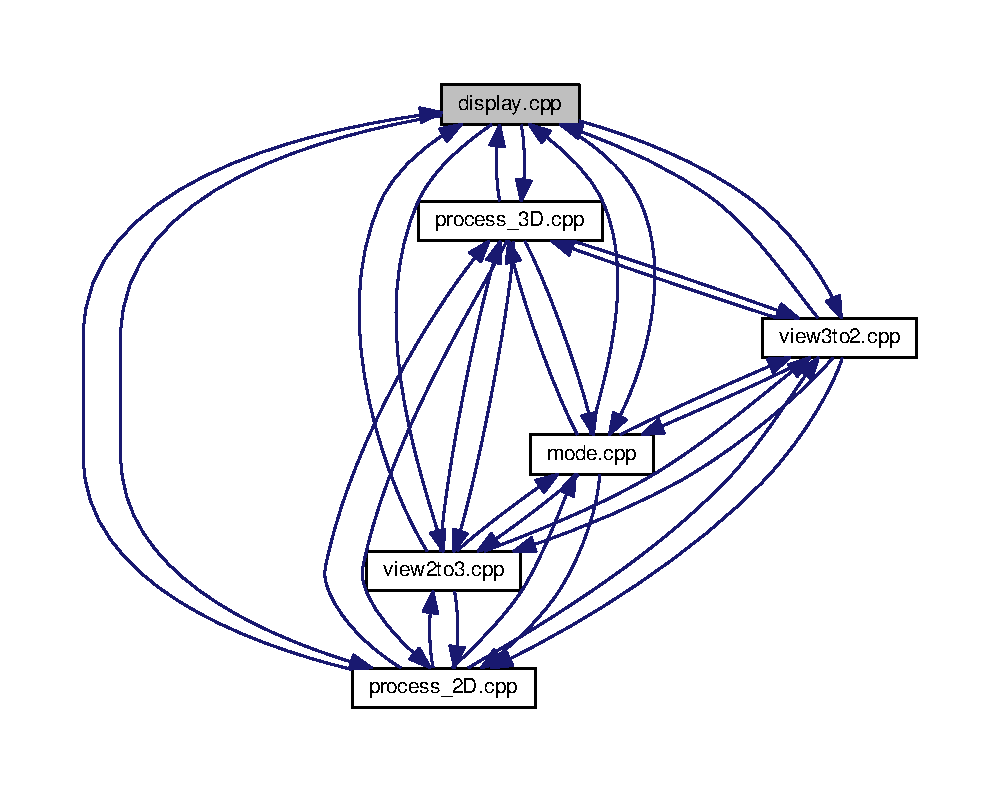
\includegraphics[width=350pt]{display_8cpp__dep__incl}
\end{center}
\end{figure}
\subsection*{Classes}
\begin{DoxyCompactItemize}
\item 
class \hyperlink{classgenerate__display}{generate\+\_\+display}
\end{DoxyCompactItemize}

\hypertarget{mode_8cpp}{}\section{mode.\+cpp File Reference}
\label{mode_8cpp}\index{mode.\+cpp@{mode.\+cpp}}
{\ttfamily \#include $<$bits/stdc++.\+h$>$}\newline
{\ttfamily \#include $<$Qt\+Gui$>$}\newline
{\ttfamily \#include $<$process\+\_\+3\+D.\+cpp$>$}\newline
{\ttfamily \#include $<$process\+\_\+2\+D.\+cpp$>$}\newline
{\ttfamily \#include $<$view2to3.\+cpp$>$}\newline
{\ttfamily \#include $<$view3to2.\+cpp$>$}\newline
{\ttfamily \#include $<$display.\+cpp$>$}\newline
Include dependency graph for mode.\+cpp\+:
\nopagebreak
\begin{figure}[H]
\begin{center}
\leavevmode
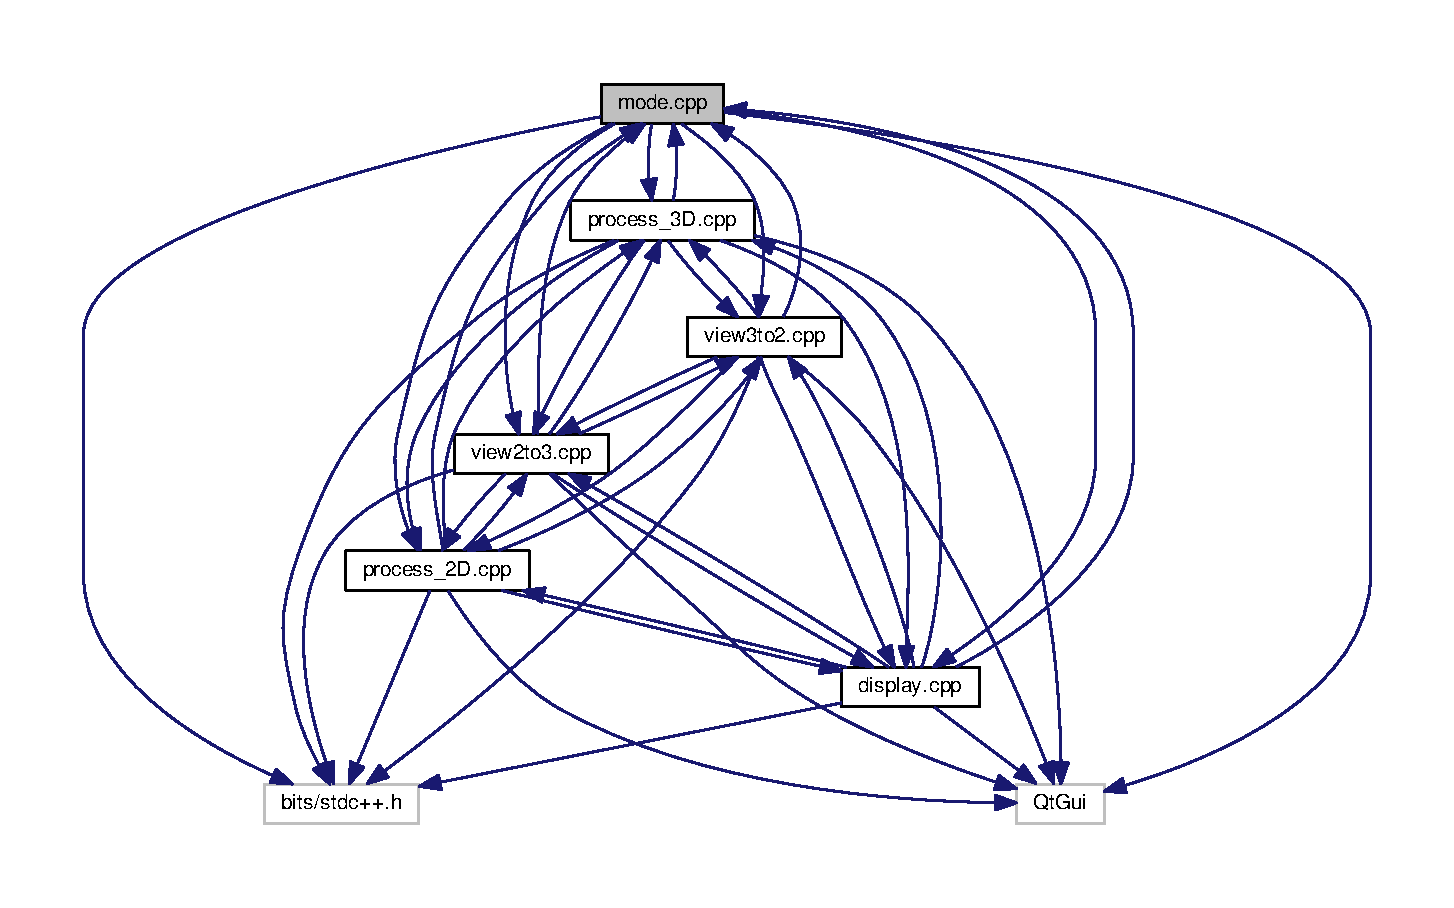
\includegraphics[width=350pt]{mode_8cpp__incl}
\end{center}
\end{figure}
This graph shows which files directly or indirectly include this file\+:
\nopagebreak
\begin{figure}[H]
\begin{center}
\leavevmode
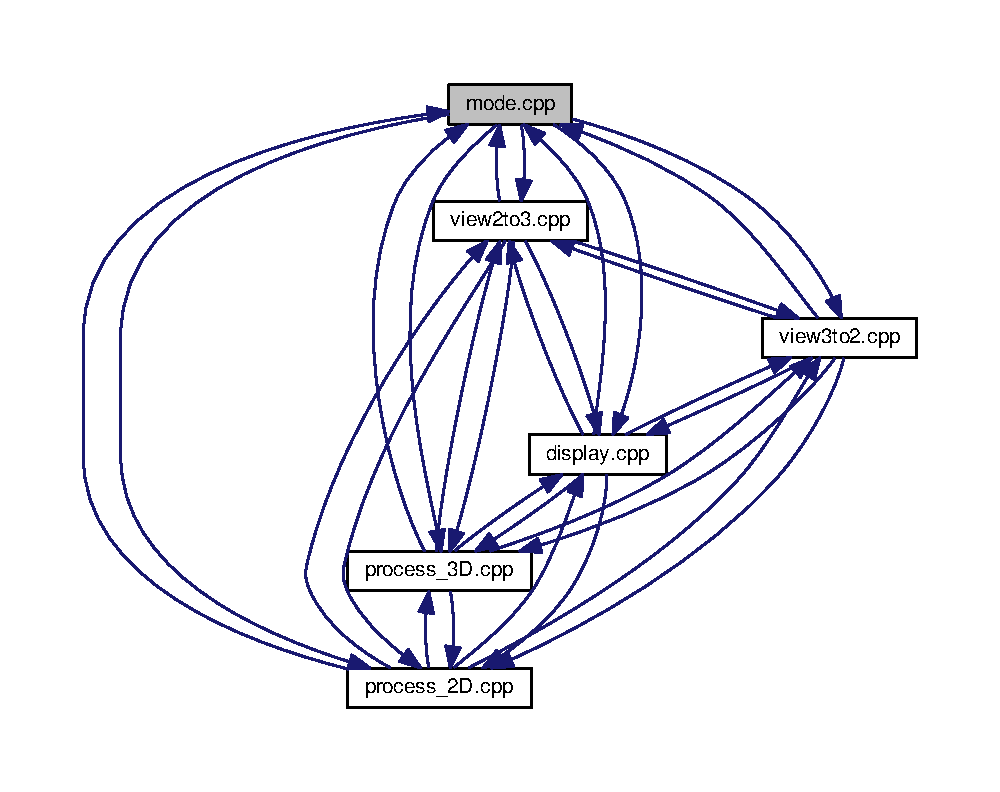
\includegraphics[width=350pt]{mode_8cpp__dep__incl}
\end{center}
\end{figure}
\subsection*{Classes}
\begin{DoxyCompactItemize}
\item 
class \hyperlink{classmode__select}{mode\+\_\+select}
\end{DoxyCompactItemize}

\hypertarget{process__2D_8cpp}{}\section{process\+\_\+2\+D.\+cpp File Reference}
\label{process__2D_8cpp}\index{process\+\_\+2\+D.\+cpp@{process\+\_\+2\+D.\+cpp}}
{\ttfamily \#include $<$bits/stdc++.\+h$>$}\newline
{\ttfamily \#include $<$Qt\+Gui$>$}\newline
{\ttfamily \#include $<$process\+\_\+3\+D.\+cpp$>$}\newline
{\ttfamily \#include $<$display.\+cpp$>$}\newline
{\ttfamily \#include $<$view2to3.\+cpp$>$}\newline
{\ttfamily \#include $<$view3to2.\+cpp$>$}\newline
{\ttfamily \#include $<$mode.\+cpp$>$}\newline
Include dependency graph for process\+\_\+2\+D.\+cpp\+:
\nopagebreak
\begin{figure}[H]
\begin{center}
\leavevmode
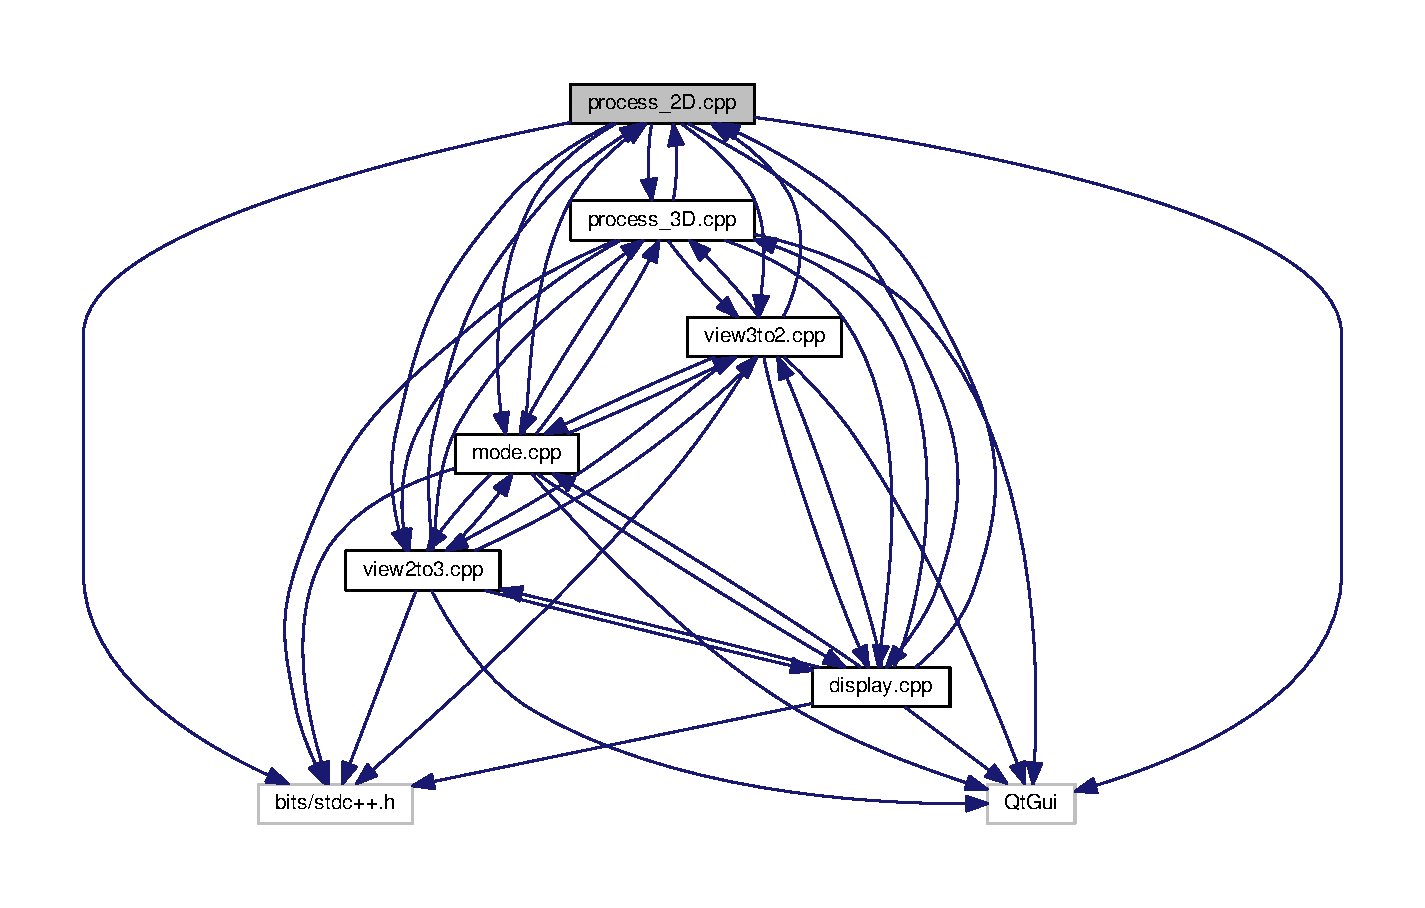
\includegraphics[width=350pt]{process__2D_8cpp__incl}
\end{center}
\end{figure}
This graph shows which files directly or indirectly include this file\+:
\nopagebreak
\begin{figure}[H]
\begin{center}
\leavevmode
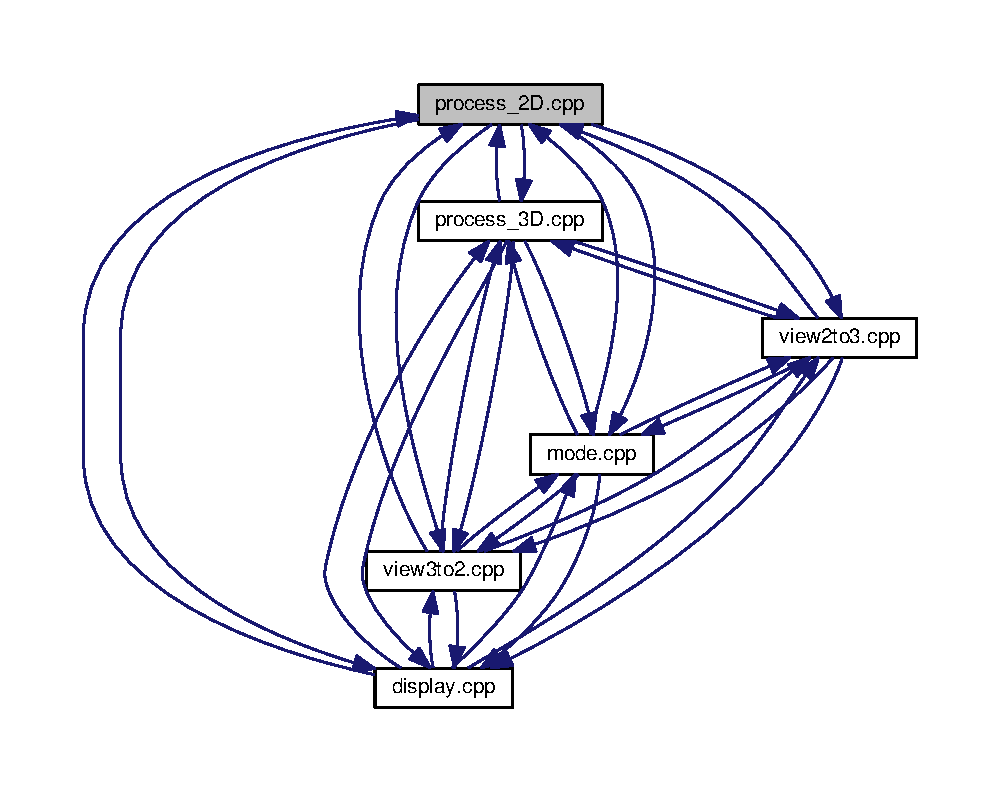
\includegraphics[width=350pt]{process__2D_8cpp__dep__incl}
\end{center}
\end{figure}
\subsection*{Classes}
\begin{DoxyCompactItemize}
\item 
class \hyperlink{classgenerate__2D}{generate\+\_\+2D}
\end{DoxyCompactItemize}

\hypertarget{process__3D_8cpp}{}\section{process\+\_\+3\+D.\+cpp File Reference}
\label{process__3D_8cpp}\index{process\+\_\+3\+D.\+cpp@{process\+\_\+3\+D.\+cpp}}
{\ttfamily \#include $<$bits/stdc++.\+h$>$}\newline
{\ttfamily \#include $<$Qt\+Gui$>$}\newline
{\ttfamily \#include $<$display.\+cpp$>$}\newline
{\ttfamily \#include $<$process\+\_\+2\+D.\+cpp$>$}\newline
{\ttfamily \#include $<$view2to3.\+cpp$>$}\newline
{\ttfamily \#include $<$view3to2.\+cpp$>$}\newline
{\ttfamily \#include $<$mode.\+cpp$>$}\newline
Include dependency graph for process\+\_\+3\+D.\+cpp\+:
\nopagebreak
\begin{figure}[H]
\begin{center}
\leavevmode
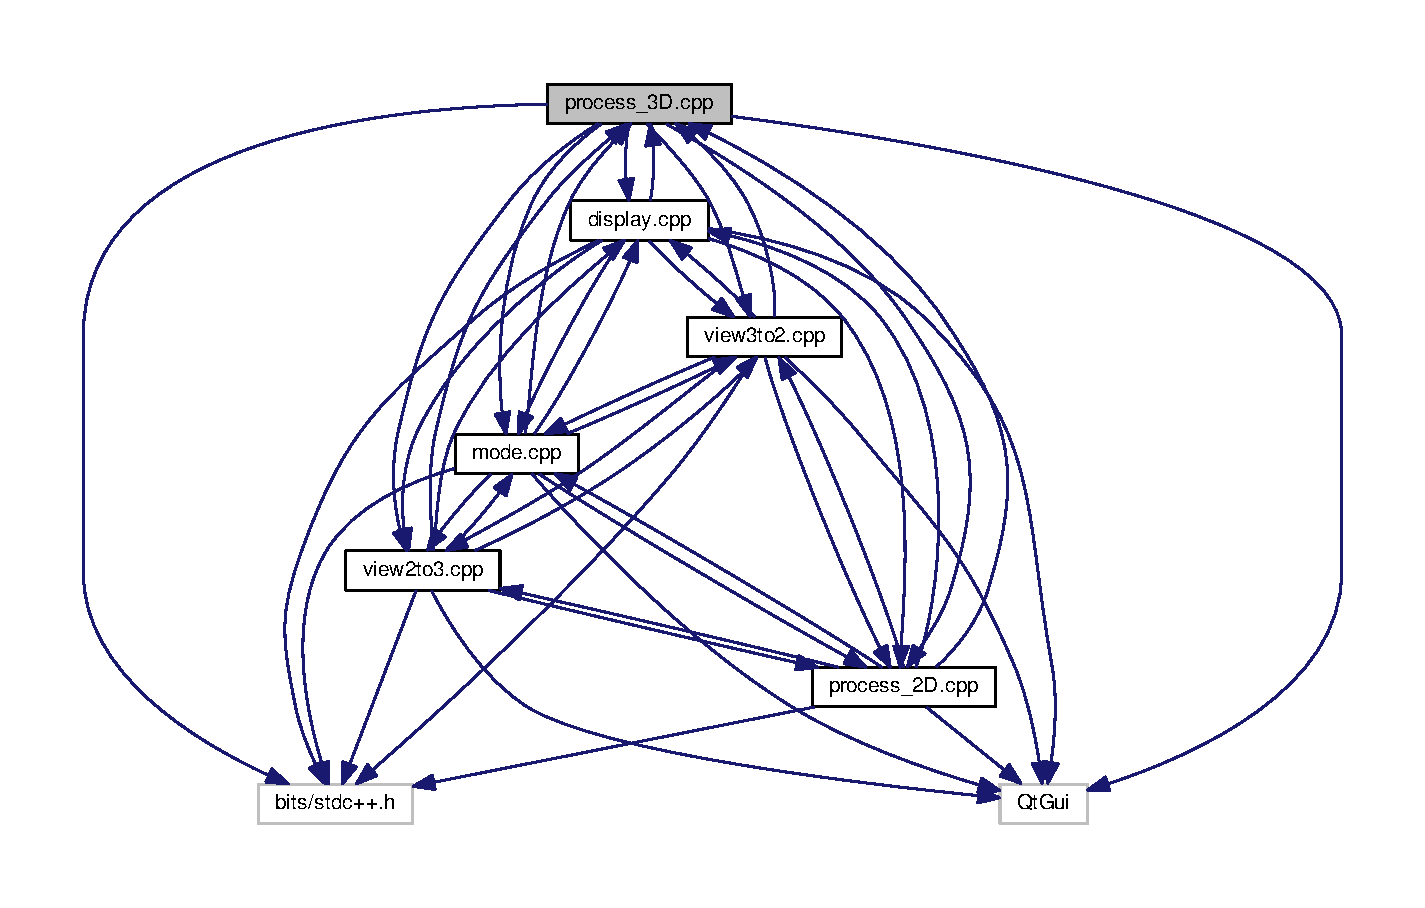
\includegraphics[width=350pt]{process__3D_8cpp__incl}
\end{center}
\end{figure}
This graph shows which files directly or indirectly include this file\+:
\nopagebreak
\begin{figure}[H]
\begin{center}
\leavevmode
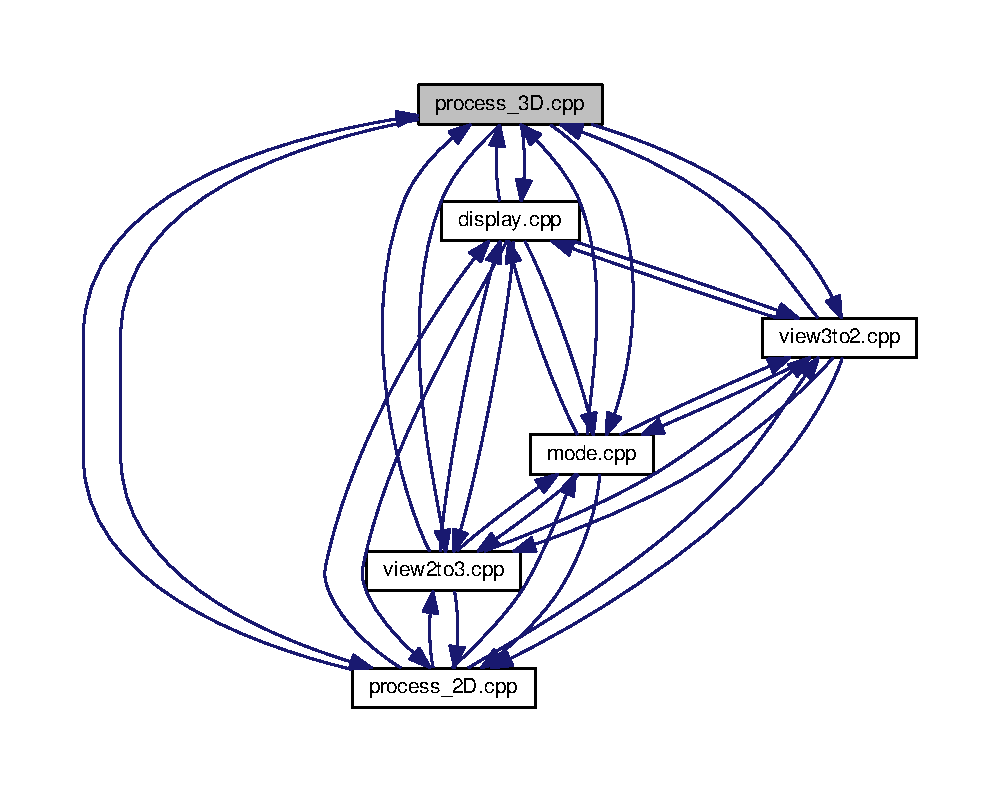
\includegraphics[width=350pt]{process__3D_8cpp__dep__incl}
\end{center}
\end{figure}
\subsection*{Classes}
\begin{DoxyCompactItemize}
\item 
class \hyperlink{classgenerate__3D}{generate\+\_\+3D}
\end{DoxyCompactItemize}

\hypertarget{view2to3_8cpp}{}\section{view2to3.\+cpp File Reference}
\label{view2to3_8cpp}\index{view2to3.\+cpp@{view2to3.\+cpp}}
{\ttfamily \#include $<$bits/stdc++.\+h$>$}\newline
{\ttfamily \#include $<$Qt\+Gui$>$}\newline
{\ttfamily \#include $<$process\+\_\+3\+D.\+cpp$>$}\newline
{\ttfamily \#include $<$process\+\_\+2\+D.\+cpp$>$}\newline
{\ttfamily \#include $<$mode.\+cpp$>$}\newline
{\ttfamily \#include $<$view3to2.\+cpp$>$}\newline
{\ttfamily \#include $<$display.\+cpp$>$}\newline
Include dependency graph for view2to3.\+cpp\+:
\nopagebreak
\begin{figure}[H]
\begin{center}
\leavevmode
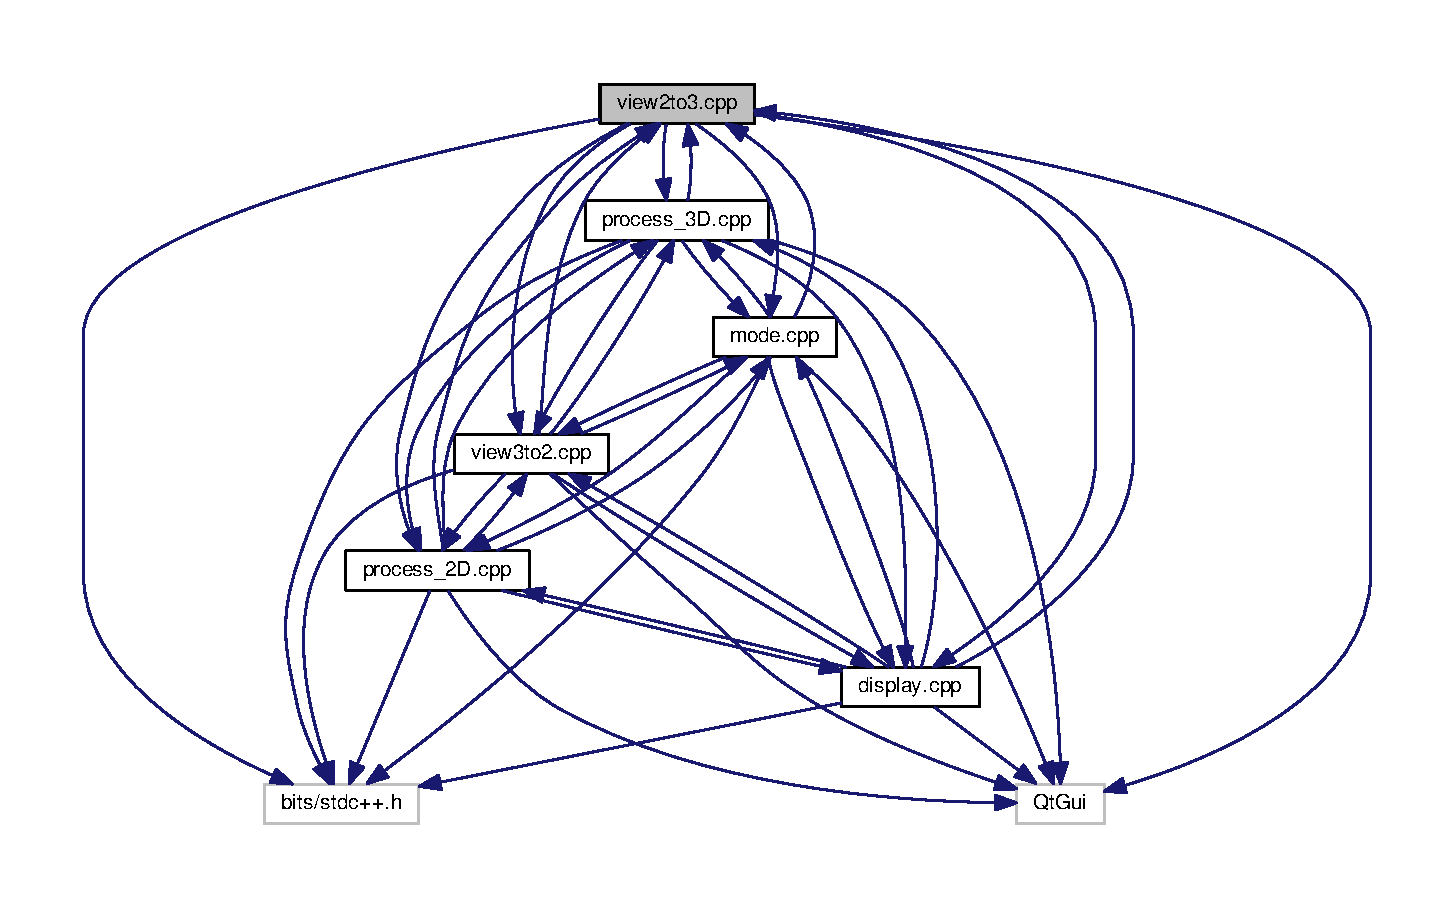
\includegraphics[width=350pt]{view2to3_8cpp__incl}
\end{center}
\end{figure}
This graph shows which files directly or indirectly include this file\+:
\nopagebreak
\begin{figure}[H]
\begin{center}
\leavevmode
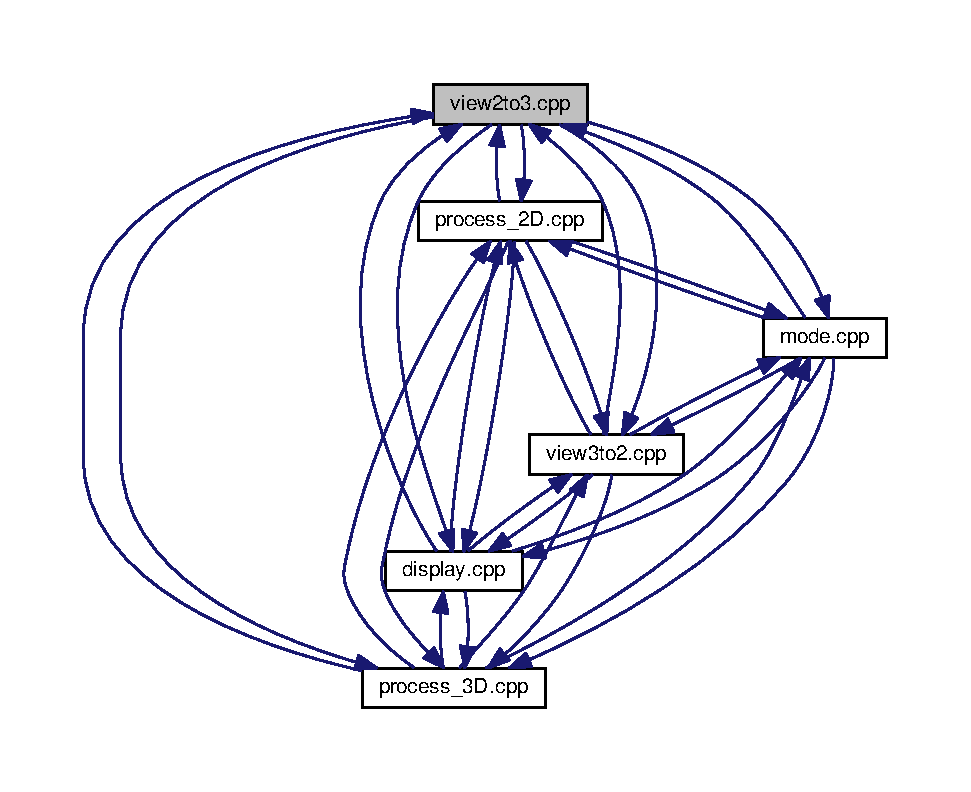
\includegraphics[width=350pt]{view2to3_8cpp__dep__incl}
\end{center}
\end{figure}
\subsection*{Classes}
\begin{DoxyCompactItemize}
\item 
class \hyperlink{classview2Dto3D}{view2\+Dto3D}
\end{DoxyCompactItemize}

\hypertarget{view3to2_8cpp}{}\section{view3to2.\+cpp File Reference}
\label{view3to2_8cpp}\index{view3to2.\+cpp@{view3to2.\+cpp}}
{\ttfamily \#include $<$bits/stdc++.\+h$>$}\newline
{\ttfamily \#include $<$Qt\+Gui$>$}\newline
{\ttfamily \#include $<$process\+\_\+3\+D.\+cpp$>$}\newline
{\ttfamily \#include $<$process\+\_\+2\+D.\+cpp$>$}\newline
{\ttfamily \#include $<$view2to3.\+cpp$>$}\newline
{\ttfamily \#include $<$mode.\+cpp$>$}\newline
{\ttfamily \#include $<$display.\+cpp$>$}\newline
Include dependency graph for view3to2.\+cpp\+:
\nopagebreak
\begin{figure}[H]
\begin{center}
\leavevmode
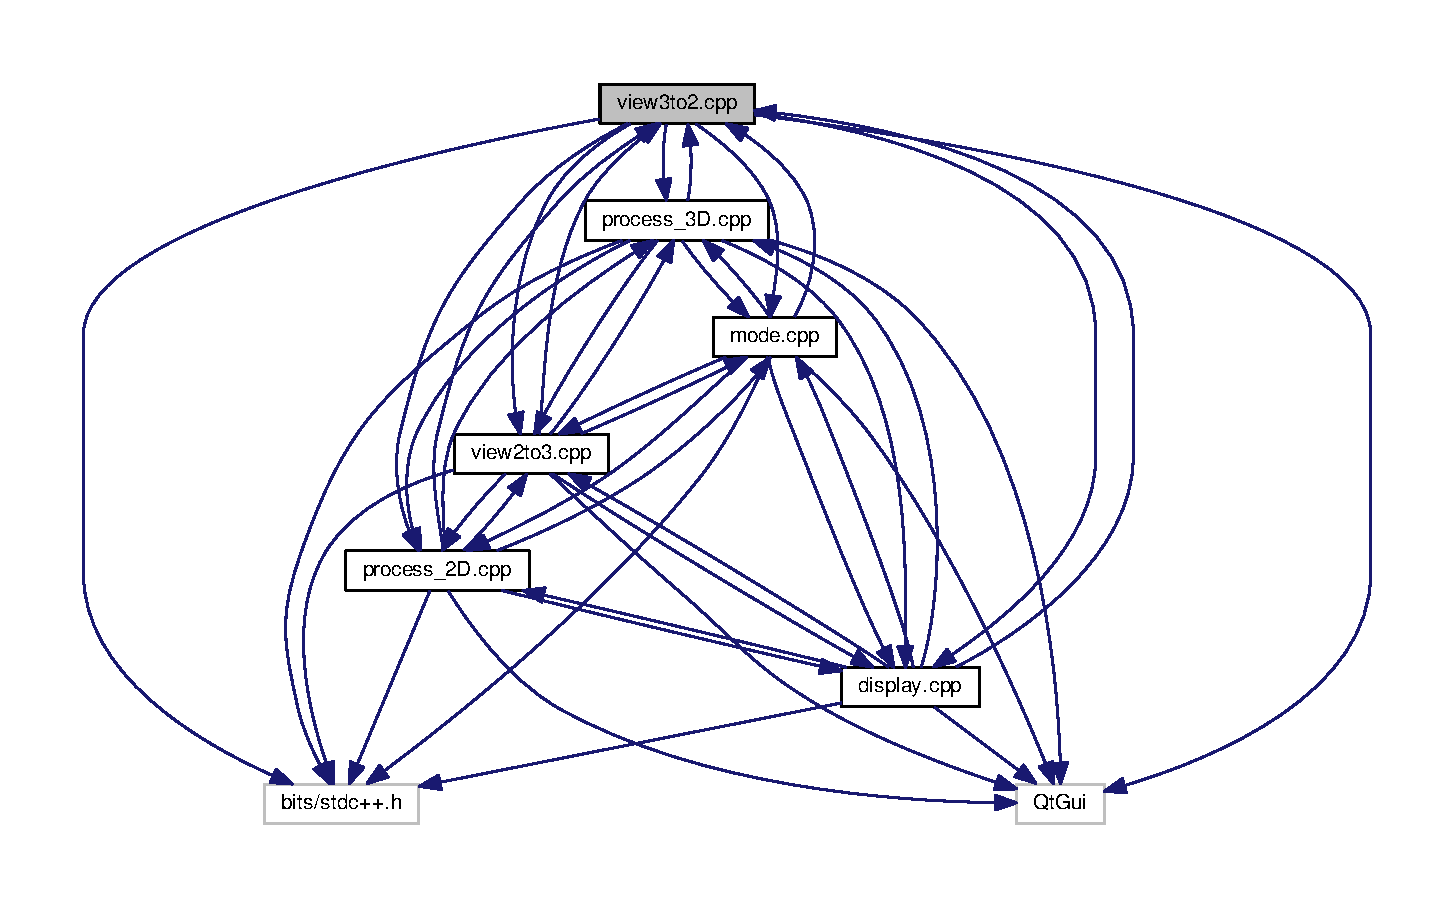
\includegraphics[width=350pt]{view3to2_8cpp__incl}
\end{center}
\end{figure}
This graph shows which files directly or indirectly include this file\+:
\nopagebreak
\begin{figure}[H]
\begin{center}
\leavevmode
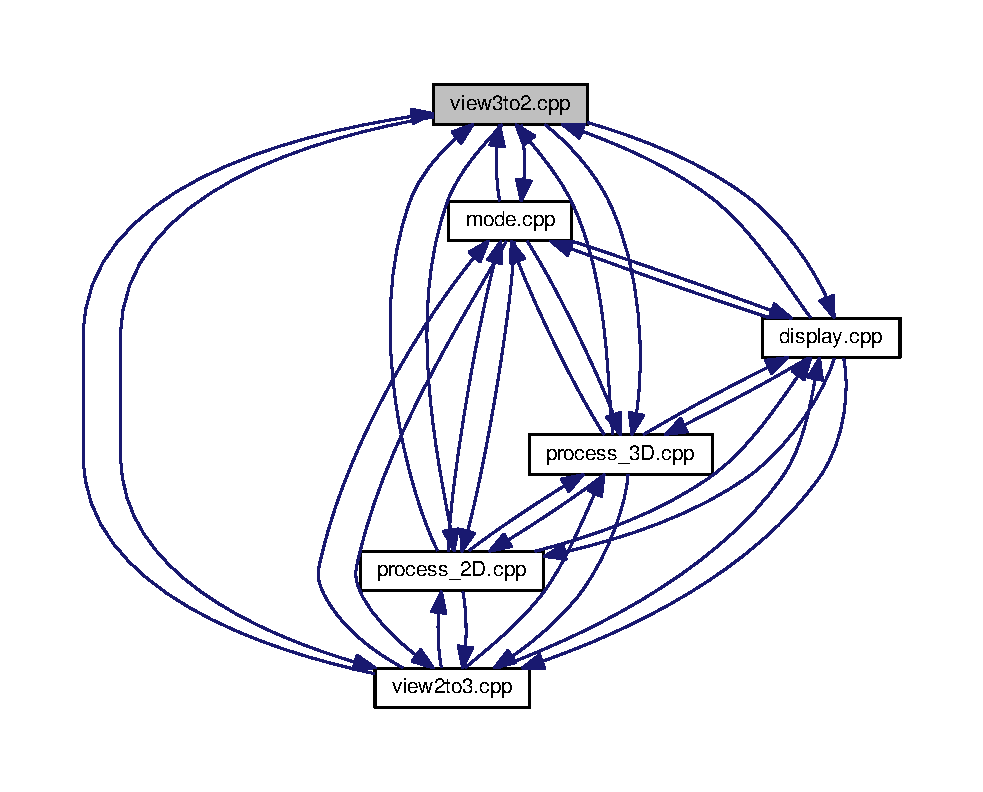
\includegraphics[width=350pt]{view3to2_8cpp__dep__incl}
\end{center}
\end{figure}
\subsection*{Classes}
\begin{DoxyCompactItemize}
\item 
class \hyperlink{classview3Dto2D}{view3\+Dto2D}
\end{DoxyCompactItemize}

%--- End generated contents ---

% Index
\backmatter
\newpage
\phantomsection
\clearemptydoublepage
\addcontentsline{toc}{chapter}{Index}
\printindex

\end{document}
